\documentclass[12pt, a4paper]{article}

% Essential Packages
\usepackage[utf8]{inputenc}
\usepackage[T1]{fontenc}
\usepackage{geometry}
\usepackage{graphicx}
\usepackage{amsmath, amssymb}
\usepackage{hyperref}
\usepackage{booktabs}
\usepackage{tabularx}
\usepackage{enumitem}
\usepackage{titlesec}
\usepackage{parskip}
\usepackage{float} % For precise figure placement
\usepackage{listings} % For code snippets
\usepackage{xcolor}
\usepackage{tikz}
\usetikzlibrary{arrows.meta, positioning, shapes, calc, backgrounds, fit}

% Geometry setup
\geometry{
    left=25mm,
    right=25mm,
    top=25mm,
    bottom=25mm
}

% Hyperlink setup
\hypersetup{
    colorlinks=true,
    linkcolor=black,
    citecolor=blue,
    urlcolor=blue
}

% Code snippet styling
\definecolor{codegray}{rgb}{0.5,0.5,0.5}
\definecolor{codepurple}{rgb}{0.58,0,0.82}
\definecolor{backcolour}{rgb}{0.95,0.95,0.92}

\lstdefinestyle{mystyle}{
    backgroundcolor=\color{backcolour},   
    commentstyle=\color{codegray},
    keywordstyle=\color{magenta},
    numberstyle=\tiny\color{codegray},
    stringstyle=\color{codepurple},
    basicstyle=\ttfamily\footnotesize,
    breakatwhitespace=false,         
    breaklines=true,                 
    captionpos=b,                    
    keepspaces=true,                 
    numbers=left,                    
    numbersep=5pt,                  
    showspaces=false,                
    showstringspaces=false,
    showtabs=false,                  
    tabsize=2
}
\lstset{style=mystyle}

% Title Metadata
\title{\textbf{Bizarre Museum: A Mixed Reality Dream Curator} \\ \large Technical Documentation \& Interaction Report}

\author{
    \textbf{Nouraldin Gaser Yousri Algendi} \\
    \textbf{Debaj Shady Elmaghraby} \\
    German International University (GIU) \\
    \textit{Course: Extended Realities (Winter 2025/2026)}
}
\date{\today}

\begin{document}

\maketitle

\begin{abstract}
Bizarre Museum is a mixed-reality prototype that bridges the gap between Mobile AR and VR. The experience gamifies the collection of "dream fragments" in the real world (AR) and allows users to curate and experiment with these fragments in a surreal virtual museum (VR). This report documents the system architecture, specifically the "Seed/DNA" data model, the interaction design implemented using Unity's UI Toolkit, and the technical implementation of the cross-platform experience.
\end{abstract}

\tableofcontents
\newpage

\section{Project Overview}
\textit{Bizarre Museum} explores the concept of object permanence and transformation across different realities. The core loop consists of two distinct phases:
\begin{enumerate}
    \item \textbf{The Collector (AR):} Users capture floating "dream bubbles" in their physical environment using a mobile device.
    \item \textbf{The Curator (VR):} Users utilize an access code to retrieve their collected items in a virtual space, where they can manipulate the items' parameters to create surreal environmental effects.
\end{enumerate}

\section{System Architecture}
The project utilizes a "Client-Authority" architecture pattern to handle the procedural generation of item behaviors.

\subsection{The "DNA Bank" Philosophy}
To allow for complex, randomized behaviors (gravity distortion, color shifting, audio synthesis) without heavy server-side computation, we implemented a \textbf{Seed-Based Architecture}.

\begin{itemize}
    \item \textbf{The Server (Node.js/Express + MongoDB):} Acts as a passive state container. It does not store physical parameters (e.g., "Gravity Force = 9.8"). Instead, it assigns a random floating-point \texttt{seed} ($0.0 - 1.0$) to every item collected.
    \item \textbf{The Client (Unity):} Acts as the "DNA Unpacker." It receives the seed and uses it to initialize a deterministic Random Number Generator (RNG). This ensures that a specific seed always produces the exact same set of complex behaviors on any device.
\end{itemize}

\begin{figure}[h]
    \centering
    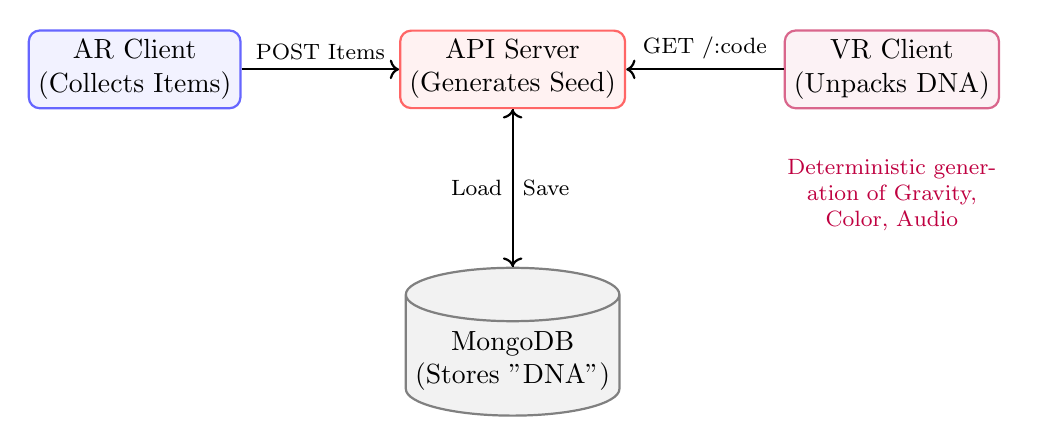
\begin{tikzpicture}[node distance=2cm, auto, thick]
        % Nodes
        \node (ar) [rectangle, draw=blue!60, fill=blue!5, rounded corners, minimum width=2.5cm, align=center] {AR Client\\(Collects Items)};
        \node (api) [rectangle, draw=red!60, fill=red!5, rounded corners, minimum width=2.5cm, right=of ar, align=center] {API Server\\(Generates Seed)};
        \node (db) [cylinder, shape border rotate=90, draw=gray, fill=gray!10, aspect=0.25, below=of api, align=center] {MongoDB\\(Stores "DNA")};
        \node (vr) [rectangle, draw=purple!60, fill=purple!5, rounded corners, minimum width=2.5cm, right=of api, align=center] {VR Client\\(Unpacks DNA)};

        % Arrows
        \draw[->] (ar) -- node[above, font=\footnotesize] {POST Items} (api);
        \draw[->] (api) -- node[right, font=\footnotesize] {Save} (db);
        \draw[->] (db) -- node[left, font=\footnotesize] {Load} (api);
        \draw[->] (vr) -- node[above, font=\footnotesize] {GET /:code} (api);
        
        % Annotations
        \node [below=0.5cm of vr, font=\footnotesize, text width=3cm, align=center, color=purple] {Deterministic generation of Gravity, Color, Audio};
    \end{tikzpicture}
    \caption{Data Flow: From AR Collection to VR Generation}
    \label{fig:arch}
\end{figure}

\section{Interaction Design \& Implementation}

\subsection{Phase 1: AR Interaction (The Collector)}
The AR phase focuses on physical movement and discovery.

\subsubsection{Bubbles \& Raycasting}
Floating "Dream Bubbles" are instantiated around the user in world space. We implemented a Raycast system that translates 2D screen taps into 3D world interactions.
\begin{itemize}
    \item \textbf{Interaction:} Tapping a bubble "pops" it, dropping the primitive item to the floor.
    \item \textbf{Collection:} Proximity triggers (Colliders) detect when the user walks over an item, adding it to the inventory.
\end{itemize}

\subsubsection{Inventory System (UI Toolkit)}
We utilized Unity's \textbf{UI Toolkit (UXML/USS)} for a performant, resolution-independent HUD.
\begin{itemize}
    \item The inventory is a flex-container that dynamically fills as items are collected.
    \item Upon collecting 3 items, the "Upload Machine" appears.
\end{itemize}

\begin{figure}[H]
    \centering
    % Ensure ar.png is in the same folder as your .tex file
    \includegraphics[width=0.8\textwidth]{ar.png}
    \caption{AR Interface: Dream Bubbles and Inventory System}
    \label{fig:ar_ui}
\end{figure}

\subsection{Phase 2: VR Interaction (The Curator)}
The VR phase shifts focus to experimentation and environment manipulation.

\subsubsection{The Login Terminal}
Upon entering the scene, the user is presented with a holographic keypad created with UI Toolkit.
\begin{itemize}
    \item The user enters the 6-character code generated in the AR session.
    \item An API call retrieves the specific configuration of items.
\end{itemize}

\subsubsection{Pedestals \& Auras}
The room contains three interactive pedestals. Placing an item on a pedestal triggers its \texttt{Configure(seed)} method.
\begin{itemize}
    \item \textbf{Gravity Anomaly:} Uses the seed to determine force magnitude and direction, physically rotating and lifting nearby objects.
    \item \textbf{Chromatic Shifter:} Uses the seed to select a color palette (Gradient) and cycle speed, affecting the materials of the room.
    \item \textbf{Humming Relic:} Uses the seed to generate audio pitch and modulation speed.
\end{itemize}

% PLACEHOLDER FOR SCREENSHOT
\begin{figure}[H]
    \centering
    % Ensure vr.png is in the same folder as your .tex file
    \includegraphics[width=0.8\textwidth]{vr.png}
    \caption{VR Museum: Items activated on pedestals showing aura effects}
    \label{fig:vr_ui}
\end{figure}

\section{Implementation Details}

\subsection{The "Unpacker" Pattern}
To ensure the same "random" behavior occurs on both the developer's machine and the user's device, we use \texttt{System.Random} initialized with the downloaded seed.

% FIX 1: language=[Sharp]C instead of language=C#
\begin{lstlisting}[language={[Sharp]C}, caption=C\# Implementation of Seed Unpacking]
public override void Configure(float seed) {
    // Convert normalized float (0.0-1.0) to integer seed
    int numericSeed = (int)(seed * 100000);
    System.Random rng = new System.Random(numericSeed);

    // Deterministically generate parameters
    float intensity = (float)rng.NextDouble(); // Always same for this seed
    float range = (float)rng.NextDouble() * 5.0f;
    
    // Apply to Aura
    auraController.SetIntensity(intensity);
    auraController.SetRange(range);
}
\end{lstlisting}

\subsection{Input Abstraction}
To facilitate rapid testing in the Unity Editor without deploying to devices constantly, we implemented an \texttt{InputAdapter} class. This wrapper intercepts input calls, automatically switching between:
\begin{itemize}
    \item \textbf{Editor Profile:} Mouse clicks for taps, WASD + Right Click for movement/look.
    \item \textbf{Device Profile:} Touch inputs (AR) and XR Controller inputs (VR).
\end{itemize}

% FIX 2: Escaped the ampersand here
\section{Conclusion \& Future Work}
The prototype successfully demonstrates a continuous data loop between AR and VR environments. The "Seed" architecture proved highly effective for synchronizing complex procedural behaviors with minimal data transfer. Future iterations will focus on replacing primitive shapes with scanned 3D assets and implementing spatial audio layers for the Humming Relic.

\end{document}